\chapter{Modstanderargumenter - teknikker, eksempler}

\section{Terminologi og Notation}%
\label{sec:terminologi}

\begin{note}[Kilder]
	\href{https://imada.sdu.dk/u/jbj/DM553/LBnoteJBJ21.pdf}{Jørgens Noter på Lower Bounds}
\end{note}

Da vi primært går ud fra Jørgens noter, og han forklarer dem til at starte med, vil jeg gøre det samme. Du kan se dette delkapitel som en form for \textit{ordbog} for resten af kapitlet.

En \textit{digraph} er en rettet graf, og skrives $D = (V,A)$ hvor $V$ er mængden af knuder og $A$ mængden af kanter (arcs). $V(D)$ er mængden af knuder og $A(D)$ mængden af kanter. En kant der går rettet fra $u$ til $v$ skrives $u \rightarrow v$. Vi siger at en kant \textit{starter} i $u$ og \textit{slutter} i $v$. For hver knude $x \in V(D)$, lader vi $d^{+}_{D}(x)$ og $d^{-}_{D}(x)$ være henholdsvis antallet af kanter der starter i $x$ og antallet af kanter der slutter i $x$. $d_{D}(x)$ er alle kanter der er incident i $x$, altså enten starter eller slutter i $x$.

En \textit{komplet graf} $K_{n}$ er en graf på $n$ knuder, hvor hver knude har en kant til alle andre knuder. Altså \(\forall u, v \in V : \exists (u,v)\). Bemærk her at en komplet graf ikke er rettet.

Et \textit{out-træ} (out-arborescence på engelsk) er en orientering af et træ således at hver knude undtagen én, som vi kalder \textit{roden}, har præcis én kant der går til den, altså $d_{D}^{-}(v) = 1 \; \forall v \in V$. Ingen kanter går til roden.

En rettet graf er \textit{acyklisk} hvis det ikke har en rettet kreds. Hvis en rettet graf $D$ på $n$ knuder er acyklisk, kan vi skrive dens knuder $v_{1}, v_{2}, \ldots, v_{n}$, således at der er ingen kant $v_{j} \rightarrow v_{i}$, hvor $i < j$.

En \textit{turnering} er en orientering af en \textit{komplet graf}, altså en komplet graf men hvor kanterne er rettet, og der må højest være én kant mellem to knuder $u, v$. Der er præcist én acyklisk turnering på $n$ knuder. Vi kalder en sådan acyklisk turnering for en \textit{transitiv turnering} på $n$ knuder, fordi den har egenskaben, at hvis $x \rightarrow y$ og $y \rightarrow z$ er kanter, så er $x \rightarrow z$ også en kant.

\section{Sortering og acykliske delvise orienteringer af $K_{n}$}%
\label{sec:jbjnotes3}

Fra de tidligere definitioner kan vi definere en transitiv turnering $TT_{n}$ til at være en graf $D = (V,A)$ hvor $|V| = n$, $V  =\{x_{1}, x_{2}, \ldots, x_{n}\}$ og $A = \{x_{i} \rightarrow x_{j} : x_{i} < x_{j}\}$. Den transitive turnering har egenskaben at hvis $x_{i} \rightarrow x_{j}$ og $x_{j} \rightarrow x_{k}$, så er $x_{i} \rightarrow x_{k}$ også en kant. Dette kommer fra at en transitiv turnering er en komplet graf.

\begin{lemma}
	Lad $M = (V, A \cup E)$ blive fundet fra den komplette graf $K_{n}$ ved at orientere en delmængde $A$ af alle kanter i $K_{n}$. Mængden $E$ er kanterne der endnu ikke er blevet tildelt en orientering til. Lad $D = (V,A)$ være en rettet graf indeholdende alle knuder i $V$ og kanterne $A$. Så kan man orientere kanterne i $E$ således at den resulterende turnering $T = (V, A \cup A')$ er acyklisk $\iff$ $D$ er acyklisk. Her er $A'$ mængden af kanter vi får ved at orientere kanterne i $E$.
\end{lemma}

Altså, det er kun muligt at lave en transitiv turnering hvis en delmængde af kanterne er acyklisk til at starte med.

Givet en acyklisk rettet graf $G = (V,A)$ med $n$ knuder $V = \{v_{1}, v_{2}, \ldots, v_{n}\}$ kan vi give en mængde $S$ af $n$ forskellige reelle tal $x_{1}, x_{2}, \ldots, x_{n}$, altså en for hver knude, med egenskaben at $x_{i} > x_{j}$ hvis og kun hvis der ikke er en rettet vej fra $v_{i}$ til $v_{j}$ i $D$.

For at gøre dette, starter vi fra en acyklisk ordning $\mathcal{L}$ af $V(D)$ og lader tallene i $S$ være arbitrære forskellige tal, som opretholder $x_{i} > x_{j}$, hvis og kun hvis $v_{i}$ kommer efter $v_{j}$ i $\mathcal{L}$. Ud fra denne definition kan vi altid lade $S$ være mængden $\{1, 2, \ldots, n\}$, ved at associerer tallet $i$ med den $i$'e knude i $\textsc{L}$.

Altså har vi vist at hver delvis orientering $M = (V, A \cup E)$ af den komplette graf $K_{n}$ svarer til en eller flere permutationer af tal $1, 2, \ldots, n$ hvis og kun hvis den orienterede del $D = ( V,A )$ er acyklisk.

Lad os give et kort eksempel, før vi går videre. Lad $n = 3$, og $V = \{v_{1}, v_{2}, v_{3}\}$. Vi kan tildele værdierne $x_{v_{2}} = 1$, $X_{v_{3}} = 2$, $x_{v_{1}} = 3$. Vi orienterer derefter kanterne således:
\begin{itemize}
	\item $v_{2} \rightarrow v_{3}$ fordi $1 < 2$
	\item $v_{3} \rightarrow v_{1}$ fordi $2 < 3$
	\item $v_{2} \rightarrow v_{1}$ fordi $1 < 3$
\end{itemize}
Disse orienteringer giver os permutationen $\{2,3,1\}$.

Vores argumenter senere angående delvise orienteringer $D$ af $K_{n}$ kan blive oversat til konkrete inputs hvilke vil tvinge den faktiske algoritme til at udføre det hævdet antal af sammenligninger, blot ved at erstatte knuderne i $D$  med tallene $\{1, 2, \ldots, n\}$ på en sådan måde at tallet $x_{k}$, altså det $k$\emph{*} tal i inputtet, er givet værdien $i$ præcis hvis knuden $v_{k} \in V$ er givet pladsen $i$ i den nuværende acykliske ordning $\mathcal{L}$ af $D$.

Vi definerer nu $Q(x,y)$ til at være spørgsmålet som spørger om en sammenligning af $x$ og $y$ af algoritmen. Vi svarer altid på en query ved at give en orientering af en kant $(x,y) \in K_{n}$. Siden ingen optimal algoritme vil sammenligne de samme to tal mere end én gang, kan vi antage at $x$ og $y$ ikke er blevet sammenlignet tidligere af algoritmen, og at de heller ikke vil blive sammenlignet senere.

Vi bruger $D$ som den faktiske orienterede graf med $n$ knuder og de kanter som endnu ikke er blevet orienteret. Dermed, vil begyndelsen have en rettet graf $D = (V, \emptyset)$. Derudover vil vi lade $\mathcal{L}(D)$ være den nuværende acykliske ordning af $D$. Ydermere, vil $\mathcal{L}_{D}(x)$ være positionen af knude $x$ i $\mathcal{L}(D)$, altså $\mathcal{L}_{D}(x) = i$ hvis og kun hvis $x$ er den $i$'e knude i $\mathcal{L}(D)$. Modstanderen vil opdatere $\textsc{L}(D)$ efter nye kanter bliver orienteret, således at det er en invariant at $\textsc{L}(D)$ er en acyklisk ordning af den nuværende rettet graf $D$.

Før vi går videre, lad os kigge på et eksempel. Antag at $n = 3$, $V = \{v_{1}, v_{2}, v_{3}\}$, $D = (V, \emptyset)$ og $\textsc{L}(D) = (v_{1}, v_{2}, v_{3})$ til at starte med.
\begin{itemize}
	\item Det første spørgsmål: $Q(1,2)$:
	      \begin{itemize}
		      \item Vi sammenligner knuderne der svarer til tal $1$ og $2$.
		      \item Hvis $1 < 2$, så $v_{1} \rightarrow v_{2}$.
	      \end{itemize}
	\item Vi opdaterer $\textsc{L}(D)$:
	      \begin{itemize}
		      \item En ny acyklisk ordning kunne være $\textsc{L}(D) = (v_{1}, v_{2}, v_{3})$ (altså ingen ændring, da $v_{1}$) allerede var før $v_{2}$.
	      \end{itemize}
	\item Næste spørgsmål $Q(1,3)$:
	      \begin{itemize}
		      \item Sammenlign knuderne.
		      \item Hvis $3 < 1$, så $v_{3} \rightarrow v_{1}$
	      \end{itemize}
	\item Vi opdaterer $\mathcal{L}(D)$:
	      \begin{itemize}
		      \item En ny acyklisk ordning ville være $\textsc{L}(D) = (v_3, v_{1}, v_{2})$.
	      \end{itemize}
	\item Næste spørgsmål $Q(3,2)$:
	      \begin{itemize}
		      \item Sammenlign knuder der svarer til tal $3$ og $2$.
		      \item Hvis $3 < 2$, orienter $v_{3} > v_{2}$.
	      \end{itemize}

	\item Opdater $\textsc{L}(D)$:
	      \begin{itemize}
		      \item En ny acyklisk ordning ville være $\textsc{L}(D) = (v_{3}, v_{1}, v_{2})$.
	      \end{itemize}
\end{itemize}

\section{Nedre grænser for minimum og maksimum blandt $n$ tal}%
\label{sec:label}

Modstanderen bygger en delvis orientering af $K_{n}$ som altid er acyklisk, ved at svare på spørgsmålet $Q(x,y)$ i forhold til den følgende strategi:
\begin{enumerate}
	\item Hvis $d_{D}^{+}(x) = 0 = d_{D}^{+}(y)$, så tilføjes kanten $x \rightarrow y$ til $D$ hvis $d_{D}^{-}(y) > y$. Tilføj kanten $y \rightarrow x$ til $D$ hvis $d_{D}^{-}(y) = 0$.
	\item Hvis $d^{+}_{D}(x) = 0 < d^{+}_{D}(y)$, så tilføjes kanten $y \rightarrow x$ til $D$.
	\item Hvis $d^{+}_{D}(x) > 0$ og enten $d_{D}^{+}(y) = 0$ eller $d_{D}^{-}(x) = 0$, så tilføjes kanten $x \rightarrow y$ til $D$.
	\item Hvis $d^{+}_{D}(x) d_{D}^{-}(x) > 0$ og $d_{D}^{+}(y) > 0$, men $d_{D}^{-}(y) = 0$, så tilføj kanten $y \rightarrow x$ til $D$.
	\item Hvis $d_{D}^{+}(x)d^{-}_{D}(x), d^{+}_{D}(y)d_{D}^{-}(y) > 0$, så tilføj kanten $x \rightarrow y$ til $D$ hvis $\mathcal{L}_{D}(x) < \textsc{L}_{D}(y)$, altså hvis $x$ kommer før $y$ i ordningen, og ellers tilføj kanten $y \rightarrow x$ til $D$.
\end{enumerate}

\begin{wrapfigure}{l}{0.5\textwidth}
	\centering
	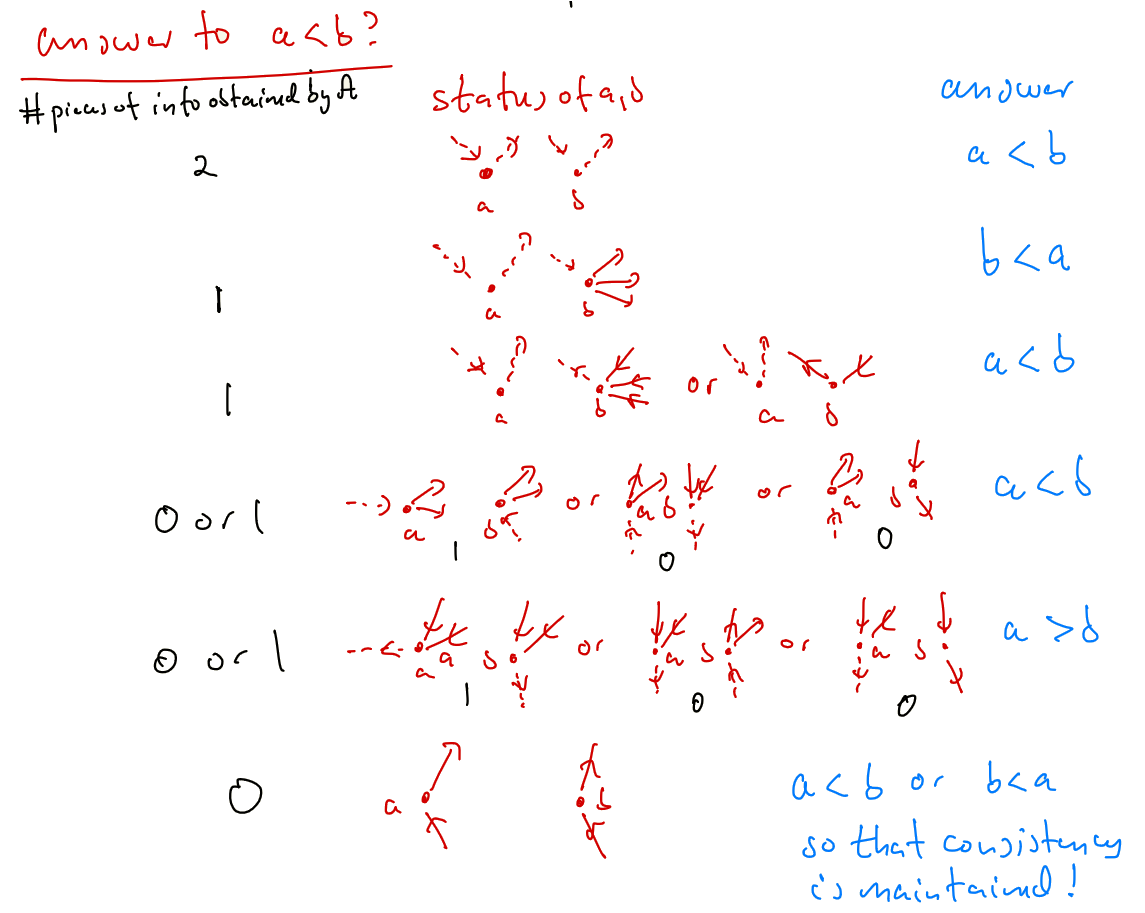
\includegraphics[scale=0.25]{figur/adversarystrategynotes.png}
	\caption{\label{fig:joergenadversarystrategi} Jørgens håndskrevne noter til modstanderens strategi.}
\end{wrapfigure}


Dette er utroligt besværligt at forstå på denne måde, så det kan også ses grafisk i Figur~\ref{fig:joergenadversarystrategi}, eller på \href{https://imada.sdu.dk/u/jbj/DM553/Slides21/Lect22.pdf}{slides til forelæsning 22 på side 5}. Lad os nu gå lidt dybere i reglerne, så vi er sikre på at vi forstår hver lille del af dem, da de egentlig er ret intuitive, når man forstår dem. De handler i bund og grund om at være sikker på at vi overholder den acykliske ordning i $\mathcal{L_{D}}$, men også at vi (som modstander) lader algoritmen få så lidt information som overhovedet muligt. Dette gør vi dog ved at opretholde den acykliske ordning, da de sikringer den giver os, sikrer os at så lidt information som muligt kommer igennem. Der er ét tidspunkt hvor algoritmen får 2 stykker information: når ingen af knuderne (elementer) er blevet sammenlignet på noget tidspunkt. Når disse bliver sammenlignet, kan vi ikke udelukke om hver element er maksimum eller minimum.

\begin{enumerate}
	\item \textbf{Regel 1}:
	      \begin{itemize}
		      \item Hvis ingen af knuderne har nogen kanter der går ud fra dem, så kigger vi på $y$, og tjekker om der går nogle kanter ud af den.
		      \item Hvis der går ingen kanter ud af $y$, så tilføjer vi kanten $y \rightarrow x$, da vi sikkert kan sige at $y < x$.
		      \item Hvis der kommer mindst én kant ud af $y$, så tilføjer vi kanten $x \rightarrow y$, da dette betyder at $y$ er større end mindst én værdi allerede, og derfor også kan være større end $x$.
	      \end{itemize}
	\item \textbf{Regel 2}:
	      \begin{itemize}
		      \item Hvis der ikke kommer nogen kanter ud af knuden $x$, men der kommer kanter ud af $y$, så tilføjer vi kanten $y \rightarrow x$ til $D$.
		      \item Da $x$ ikke har nogen udgående kanter, betyder det at $y$ må være mindre end $x$.
	      \end{itemize}
	\item \textbf{Regel 3}:
	      \begin{itemize}
		      \item Hvis der går en eller flere kanter ud fra $x$, og der enten går 0 ud fra $y$ eller 0 ind i $x$, så tilføjer vi kanten $x \rightarrow y$ til $D$.
		      \item Hvis $x$ har udadgående kanter, og $y$ ikke har nogen udadgående, betyder det at $x$ sikkert kan sættes til at være mindre end $y$.
		      \item  På samme måde, hvis der ikke kommer nogen kanter ind i $x$ betyder det at den ikke har vundet nogen kampe, og der kan derfor sagtens bliver puttet en kant til fra $x$ til $y$.
	      \end{itemize}
	\item \textbf{Regel 4}:
	      \begin{itemize}
		      \item Hvis $x$ har både kanter indadgående og udadgående og $y$ har udadgående kanter, men ingen indadgående, så kan vi sikkert tilføje $y \rightarrow x$ til $D$.
		      \item Hvis $y$ ingen indadgående kanter har, så har den tabt alle kampe indtil videre. Hvis vi bliver ved med at sige at den har tabt til $x$, sker der ingen ændring.
	      \end{itemize}
	\item \textbf{Regel 5}:
	      \begin{itemize}
		      \item Hvis både $x$ og $y$ har kanter der går både ind og ud, så gør vi som følger:
		      \item Tilføjer kanten $x \rightarrow y$ til $D$ hvis $x$ kommer før $y$ i den acykliske ordning $\textsc{L}_{D}$.
		      \item Ellers omvendt.
	      \end{itemize}
\end{enumerate}


\begin{lemma}
	Hvis $D$ er acyklisk og kanten $(x,y)$ er orienteret som over, så er den resulterende rettet graf også acyklisk.
\end{lemma}

\begin{proof}
	Det er nok her at vise at den nye kant ikke kan være en del af en kreds. I regel 1 kan $x\rightarrow y$ ikke være en del af en kreds, da $y$ ikke har nogen kanter der går ud fra sig. Det samme argument gælder i regel 2 ved $y \rightarrow x$. I regel 3 har vi enten at $y$ ikke har nogen udadgående kanter, eller $x$ ikke har nogen indadgående kanter, hvilket betyder at $x \rightarrow y$ ikke kan være en del af en kreds. Regel 4 siger at $y$ ikke må have nogen indadgående kanter, og $y \rightarrow x$ kan derfor ikke lave en kreds. I regel 5 tilføjer vi en kant således at den går fremad i forhold til den acykliske ordning, og derfor kan den ikke være en del af en kreds.
\end{proof}

Alle algoritmer der finder både maksimum og minimum blandt $n$ forskellige tal skal bruge mindst $2n-2$ stykker information. Dette kommer fra at den skal ekskludere $n-1$ tal fra at være hhv. minimum og maksimum. Det eneste tidspunkt modstanderen tvinges til at give 2 stykkre information er når den tager regel 1 i brug, som er når der er ingen indadgående kanter for begge knuder. Når regler 2 til 4 bliver taget i brug gives der højest et stykke information. Når regel 5 tages i brug gives der ingen ny information.

\begin{theorem}
	Hver algoritme som finder både maksimums- og minimumselementet blandt $n$ forskellige heltal  skal bruge mindst $\left \lceil \frac{3n}{2} \right \rceil -2$ sammenligninger.
\end{theorem}

\begin{proof}
	Lad $A$ være en arbitrær algoritme der løser problemet. ved at orientere $K_{n}$ imens $A$ kører ifølge reglerne over, vil modstanderen give 2 stykker nyt information \textbf{højest} $\lfloor n/2 \rfloor$ gange. Dermed, for at $A$ kan få al informationen som $A$ skal bruge, skal der mindst laves $2n-2-\lfloor n/2 \rfloor = \lceil 3n/2 \rceil -2$ sammenligninger.
\end{proof}

\section{Nedre grænser for at finde det andet mindste element blandt $n$ forskellige tal}%
\label{sec:label}

Vi kan ved hjælp fra en turneringsmetode (som ikke har noget at gøre med en graf-turnering) finde både minimumselementet og andet-minimumselementet på $n + \lceil \log n \rceil - 2$ sammenligninger. Vi vil nu vise, at det ikke er muligt at gøre det bedre end den metode.

Modstanderen laver en acyklisk delvis orientering af $K_{n}$, som starter fra $D = (V, \emptyset)$ ved at svare på spørgsmål af formen $Q(x,y)$ som følger. Modstanderen vedligeholder en samling af disjunkte ud-træer $T_{1}, T_{2}, \ldots, T_{k}$ (som er træer med en rod $u$, som har præcis en vej fra $u$ til en anden knude $v$. Dermed er den også acyklisk og $d_{D}^{-}(u) = 0$). Hver knude $x$ hvor $d_{D}^{-}(x) = 0$ er roden af et af ud-træerne, som vi også kan skrive $T(x)$. I begyndelsen er hver knude roden i et ud-træ, hvor roden er den eneste knude, altså $\forall v_{i} \in V : V(T(v_{i})) = \{v_i\}$.

Vi skelner mellem to forskellige typer kanter: sorter kanter og røde (prikkede) kanter. Sorter kanter svarer til kanter i træerne, og røde kanter svarer til katnerne i resten af $D$. Altså kan sort kant være minimumsværdien, og rød kant kan være andenminimum. Modstanderen følger følgende regler:

\begin{enumerate}
	\item Hvis $d_{D}^{-}(x) = d_{D}^{-} = 0$, så er både $y$ og $x$ rødder i ud-træer. Vi tilføjer en sort kant $x\rightarrow y$ hvis der er flere kanter i $T(x)$, og ellers tilføjer vi $y \rightarrow x$ hvis der er flere kanter i $T(y)$. Dermed fjerner dette også enten $x$ eller $y$ som rod.
	\item Hvis $d_{D}^{-}(x) = 0 < d_{D}^{-}(y)$, så er $x$ en rod, men $y$ er ikke, og vi kan tilføje en rød kant $x \rightarrow y$.
	\item Hvis $d_{D}^{-}(y) = 0 < d_{D}^{-}(x)$, så tilføjer vi en rød kant $y \rightarrow x$ til $D$.
	\item Hvis $d_{D}^{-}(x), d_{D}^{-}(y) > 0$ så tilføjer vi en rød kant $x \rightarrow y$ til $D$ hvis der ikke er nogen direkte $(y,x)$ vej i $D$, og ellers tilføje vi en rød kant $y \rightarrow x$ til $D$.
\end{enumerate}

\begin{lemma}
	Hvis $D$ er acyklisk og kanten $(x,y)$ er orienteret ifølge reglerne, så er den resulterende rettet graf (som vi får ved at tilføje en ny kant til $D$) stadig acyklisk og de sorte kanter laver en skov af ud-træer.
\end{lemma}
\begin{proof}
	Den sidste påstand kommer fra faktum at en ny sort knt altid vil starte i roden af et sort ud-træ til roden af et andet ud-træ. Ingen af reglerne 1-3 kan resultere i en cyklus efter vi tilføjer en ny kant, da kanterne altså vil starte i en knude $z$ hvor $d_{D}^{-}(z) = 0$. I regel 4 orienterer vi på en sådan måde at $D$ plus den nye kant vi tilføjer stadig er acyklisk, da, da $D$ er acyklisk tidligere, vil den enten have en $(x,y)$ vej eller en $(y,x)$ vej, men ikke begge.
\end{proof}

\begin{theorem}
	Ved at bruge reglerne beskrevet tidligere, vil modstanderen tvinge enhver sammenligningsbaseret algoritme $\mathcal{B}$ til at bruge mindst $n + \lceil \log n \rceil - 2$ sammenligninger til at kunne bestemme det andet mindste element.
\end{theorem}

\begin{proof}
	Lad $\mathcal{B}$ være en arbitræt sammenligningsbaseret algoritme for problemet. Så længe en knude $x$ har $d_{D}^{-}(x) = 0$, så er $x$ kandidat for at være minimumselement. Så snart $x$ får bare én kant der går ud af sig, så kan $x$ ikke længere være minimum. Dermed når $\mathcal{B}$ stopper vil der altid være præcis en knude $x$ hvor $d_{D}^{-}(x) = 0$. Det følger fra reglerne over at en knude $z$ kun kan skifte fra at have ingen kanter ind i sig, til at have mindst en når en sort kant er tilføjet til knuden. Dermed følger det fra induktion at den ene knude $x$ som har $d_{D}^{-}(x) = 0$ når $\mathcal{B}$ stopper er roden af det resulterede ud-træ, som indeholder alle $n$ knuder i $D$.

	Alle knuder i dette ud-træ, som er børn af $x$ er kandidater  til at være det andet mindste element efter at have lavet alle sammenligningerne svarende til sorte kanter. Dette kommer fra faktum at den eneste knude der kan komme til dem, udover dem selv, ved en rettet vej kun ved brug af sorte kanter er $x$. Dermed kan en sådan knude kan blive eksluderet fra et ende på andenpladsen i den endelige acykliske ordning ved at have en rød kant i sig. Hver gang en sort kant tilføjes, bliver størrelsen af det resulterende sorte ud-træ mindst fordoblet. Dermed har $x$ været roden i mindst $\lceil \log n \rceil$ forskellige ud-træer igennem kørslen af $\mathcal{B}$ og dermed har $x$ mindst $\lceil \log n \rceil$ børn i det endelige ud-træ.

	Det følger fra reglerne 1-4 at hvis $z$ har en rød kant i sig, har $z$ også en sort kant i sig. For at sikres at kun én af børnene af $x$ kan være nummer to i den endelige acykliske ordning skal mindst $t-1$ røde kanter genereres, hvor $t$ er antallet af børn i $x$ i det endelige ud-træ, som indeholder præcis $n-1$ sorte kanter når $\mathcal{B}$ stopper. Dermed skal $\mathcal{B}$ bruge mindst $(n-1) + (\lceil \log n \rceil -1) = n + \lceil \log n \rceil -2$ sammenligninger for at kunne bestemme det andet største element.
\end{proof}





%%% Local Variables:
%%% mode: latex
%%% TeX-engine: xetex
%%% TeX-command-extra-options: "-shell-escape"
%%% TeX-master: "main"
%%% End:
